\section{Forsøgte metoder}
Hvis man ser på en række vesikler, er det tydeligt at de ikke er ens. De har forskellig størrelse, både i kantens tykkelse og i diameteren. To eksempler på vesikler er vist i figur \ref{fig:premethod_ves1}, hvor det fremgår at de begge er relativt cirkulære. At vesiklerne er meget forskellige fremgår da også tydeligt af figuren. Selvom begge har nogenlunde samme farve kant, har vesiklen til venstre et meget lyst indre, hvor vesiklen til højre er meget mørkere. 

I introduktionen talte vi om hvor meget støj der var omkring alle vesiklerne, og hvordan det derfor var svært at se overgangen i kanterne. Det er derfor klart at der skal være en form for udglatning af billedet for at undertrykke støjen, og om muligt også et filter der kan fremhæve de interessante værdier.

\begin{figure}[H]
	\begin{minipage}[b]{0.5\linewidth}
		\centering
		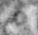
\includegraphics[scale=5]{files/premethod/img/ves1.png}
	\end{minipage}
	\hspace{0.5cm}
	\begin{minipage}[b]{0.5\linewidth}
		\centering
		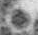
\includegraphics[scale=5]{files/premethod/img/ves2.png}
	\end{minipage}
	\caption{To udsnit af en enkelt vesikel. Begge vesikler er relativt cirkulære.\label{fig:premethod_ves1}}
\end{figure}

\subsection{Metoderne}	
At vesiklerne har fællestræk men alligevel er så forskellige, antyder at en enkelt metode ikke vil finde alle vesiklerne, og at vi i stedet skal kombinere flere metoder der tilsammen kan finde alle typer af vesikler.

Det faktum at nogen af vesiklerne er relativt cirkulære, giver os ideen at detektere cirkler i billedet. Til dette benytter vi os af Hough cirkeldetektion. Metoden er forklaret nærmere i afsnit \ref{premethod_hough}, men for at metoden kan fungere, skal billedet behandles først. Her benytter vi et Gauss filter der udglatter billedet før et sobel filter finder retninger i billedet som en kantdetektor bruger til at finde hvor der er kanter i billedet. Hver af disse funktioner er forklaret nærmere nedenfor, og vi vil til slut evaluere på resultatet.

\subsubsection{Gaussisk blur}
Et gaussisk blur, eller gaussisk udglatning, er i virkeligheden et lavpasfilter da funktionen i virkeligheden reducerer billedets højfrekvens værdier. Filteret bliver typisk brugt til at reducere billedstøj og udglatte områder. Dette er hvad vi er interesseret i, for at fjerne noget af støjen omkring vesiklerne, samtidig med at glatte kanten lidt ud så den blive glattere. I to dimmensioner er ligningen for en gaussisk funktion givet ved ligningen
\begin{align}
	G(x,y) = \frac{1}{2\pi\sigma^2}e^{-\frac{x^2+y^2}{2\sigma^2}}\label{ali:premethod_gaussG}
\end{align}
hvor x er distancen fra origo på den horisontale akse, y er distancen fra origo på den vertikale akse og $\sigma$ er standard afvigelsen af den gaussike fordeling. Når man omtaler størrelsen på den gaussiske kerne er det størrelsen på dimensionen for $G$ der bygges. Ser vi på (\ref{ali:premethod_gaussG}) så er det kun eksponentialdelen der ændrer sig når x og y ændres. Vi ser så at et større x og y får eksponentialdelen til at gå mod 0. At hæve $\sigma$ værdien vil betyde at eksponentialdelen går langsommere mod 0. Der er ikke nogen grund til at lave en matrix med den gaussiske fordeling større end dens indgange har værdier på tal større end 0. Da vi er ude efter at udglatte billeder med vesikler på størrelse med ca. 20x20 pixels, ønsker vi at bygge et gaussisk fordelingsmatrix en smule større end dette, f.eks. på 30x30 pixels. Vi vælger derfor et $\sigma$ der gør at $G(30,30) > 0$. I figur \ref{fig:premethod_gauss_table} ses en oversigt over $G(30,30)$ med $\sigma$ værdier varierende fra 5 til 15. Det ses at $\sigma$ værdier på 5-10 er meget lave, og vi vælger derfor $\sigma$ til at have værdien 15.  
 
\begin{figure}[H]
	\centering
	\begin{tabular}{l | l}
			\textbf{$\sigma$} & $G(30,30)$\\
			\hline
			$5$ & $1.476654096\cdot10^{-18}$\\
			$6$ & $6.139819206\cdot10^{-14}$\\
			$7$ & $3.425994239\cdot10^{-11}$\\
			$8$ & $1.942558050\cdot10^{-9}$\\
			$9$ & $2.936573462\cdot10^{-8}$\\
			$10$ & $1.964128034\cdot10^{-7}$\\
			$11$ & $7.740076025\cdot10^{-7}$\\
			$12$ & $0.000002133620264$\\
			$13$ & $0.000004582712125$\\
			$14$ & $0.000008229144803$\\
			$15$ & $0.00001295566429$
	\end{tabular}
	\caption{Tabel over gaussisk fordeling i pixel 30,30 efter forskellige $\sigma$ værdier.\label{fig:premethod_gauss_table}}
\end{figure}

I figur \ref{fig:premethod_gauss} ses et eksempel hvor et billede er blevet udglattet med et gauss filter. 

\begin{figure}[H]
	\begin{minipage}[b]{0.5\linewidth}
		\centering
		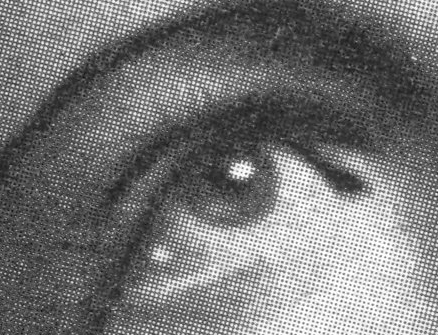
\includegraphics[scale=1.5]{files/premethod/img/gauss_pre.png}
	\end{minipage}
	\hspace{0.5cm}
	\begin{minipage}[b]{0.5\linewidth}
		\centering
		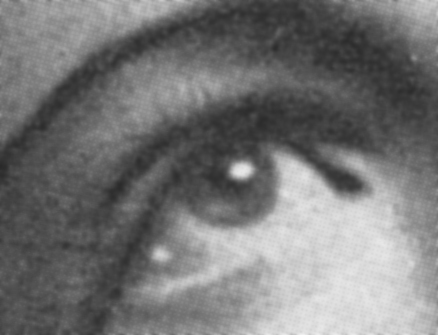
\includegraphics[scale=1.5]{files/premethod/img/gauss_post.png}
	\end{minipage}
	\caption{Billede før og efter en Gauss udglatning.\label{fig:premethod_gauss}}
\end{figure}

%VORES BILLEDE OG KOMMENTAR


\subsubsection{Sobel filter og kantdetektion}
% Behandlet fordi? res?
I billedbehandling benyttes Sobel operatoren især i kant detektion. Operatoren udregner gradienten for hvert punkt i billedet. Gradienten i et billede er en retningsændring i intensitet eller farve i et billede. Det resulterende billede indeholder så retningen i den størst mulige ændring fra lys til mørk. Jo lysere en pixel er, jo større sandsynlighed er der for at den er en del af en kant. Et eksempel på et billede der er blevet behandlet med et sobelfilter ses i figur \ref{fig:premethod_sobelres}

\begin{figure}[H]
	\begin{minipage}[b]{0.5\linewidth}
		\centering
		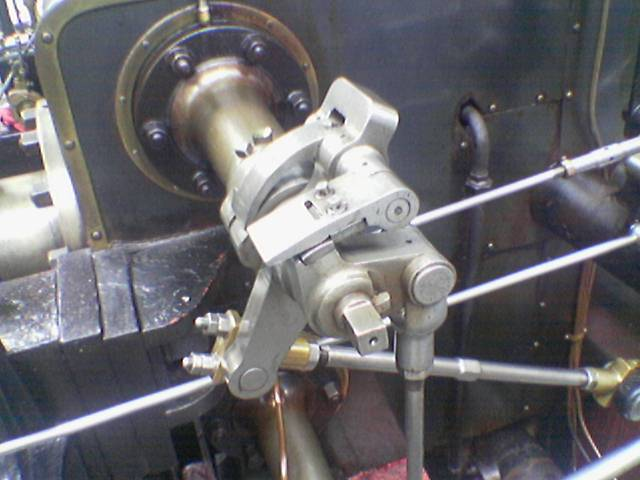
\includegraphics[scale=0.25]{files/premethod/img/sobel1.PNG}
	\end{minipage}
	\hspace{0.5cm}
	\begin{minipage}[b]{0.5\linewidth}
		\centering
		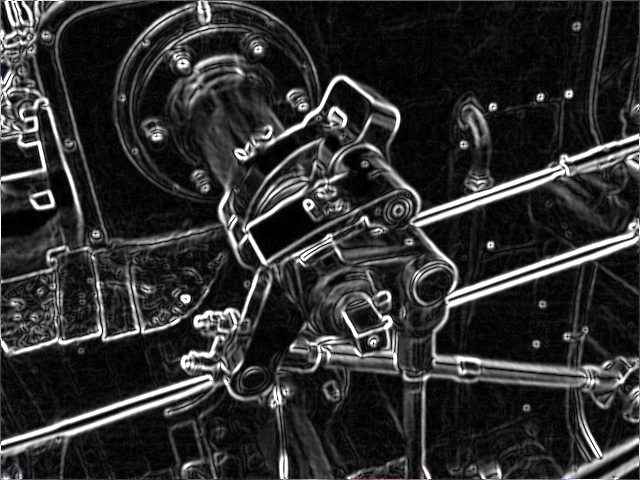
\includegraphics[scale=0.25]{files/premethod/img/sobel2.PNG}
	\end{minipage}
	\caption{Originalbilledet til venstre, og behandlet med et sobel filter til højre.\label{fig:premethod_sobelres}}
\end{figure}

At beregne et billede der er blevet behandlet med et sobelfilter er ikke særlig dyrt i forhold til udregninger, da operatoren baserer sig på at folde billedet med et lille separabel integer filter først i horisontal og så i vertikal retning. Hver af filtrene repræsenterer sin egen retning, så $G_x$ er defineret som hvordan gradienten ændrer sig i højregående retning, og $G_y$ er hvordan gradienten ændrer sig i nedadgående retning. $G_x$ og $G_y$ defineret i  (\ref{ali:premethod_sobelG}), hvor $I$ repræsenterer originalbilledet der foldes med, og $*$ operatoren betyder foldning.

\begin{align}
	G_y = \begin{bmatrix}
		-1 & -2 & -1\\
		0 & 0 & 0\\
		1 & 2 & 1
	\end{bmatrix} * I
	&&
	G_x = \begin{bmatrix}
		-1 & 0 & 1\\
		-2 & 0 & 2\\
		-1 & 0 & 1
	\end{bmatrix} * I
	\label{ali:premethod_sobelG}
\end{align} 

Det resulterende sobel billedes fås ved formlen 
\begin{align}
	G = \sqrt{G_x^2 + G_y^2}
\end{align}

På ethvert tidspunkt kan vi så finde retningen som kanten har i enhver pixel ved 
\begin{align}
	\Theta = \arctan\left(\frac{G_y}{G_x}\right)
	\label{ali:premethod_sobelTheta}
\end{align}
hvor $\Theta$ er 0 for en vertikal kant med mørkt på den venstre side. Vi skal bruge disse formler senere når vi ser på Hough cirkel detektionen der benytter sig af sobelfilteret når det skal finde kanter. 

%RESULTERENDE SOBEL PÅ VESIKLEN OG SNAK OM RESULTATET...

Ved en udvalgt tærskelværdi vil det resulterende sobel billede kun fremstå med værdi større end 0 i de pixels man med stor tiltro mener er en kant. 


\subsubsection{Hough detektion}\label{premethod_hough}
I de tidligere afsnit har vi vist hvordan vi har udglattet billedet, fundet kanter og retninger i hver af disse kanter. Disse resultater vil vi nu benytte til at finde cirklernes centrum. I (\ref{ali:premethod_sobelG}) har vi fundet $G_x$ og $G_y$ som jo var gradienterne i horisontal og vertikal retning. Vi fandt også $\theta$ i (\ref{ali:premethod_sobelTheta}), der er vinklen på en kant i den givne pixel. Vi har i vores observationer af vesiklerne også fundet ud af at de kan variere i størrelse fra 15x15 pixel, og op omkring 30x30 pixels.

Ideen er så at tage hver pixel der har en værdi større end 0 i kantbilledet efter tærskelværdien, altså hver pixel der menes at ligge på en kant, og tegne en linje ud fra denne. Linjen tegnet i en nyt canvas på samme størrelse som det originale billede, og hver pixel linjen går igennem, ligges en farveværdi oveni. Hvis hver linje så har en farveværdi på 10, og der så er 20 linjer der alle går igennem samme punkt, vil dette punkt få en farveværdi på 200. Man kan så tage en tærskelværdi på dette billede, og tilbage vil være de punkter der gerne skulle være centrum i en cirkel. 

Da vi ved at en vesikel har radius på min og maks hhv. 7.5 og 15, og vi kender $\theta$ kan vi nemt udregne ligningen for linjen der står vinkelret på punktet [i,j] (der menes at være et punkt på en kant) og har minimumsradius på 7.5 og maksimumsradius på 15. En af disse linjer ses i figur \ref{fig:premethod_houghLines}. 

\begin{figure}[H]
	\centering
	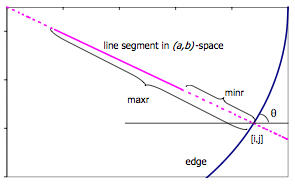
\includegraphics[scale=1]{files/premethod/img/hough_lines.png}
	\caption{Linje tegnet ud fra pixel [i,j] der menes at ligge på en kant.\label{fig:premethod_houghLines}}
\end{figure}

I figur \ref{fig:premethod_houghres} ses 4 billeder. Den første er bare en normal cirkel vi ønskes at detektere. I det andet billede er så tegnet nogle af de linjer der går igennem et punkt på kanten af cirklen samt centrum af cirklen. Her har vi ikke bekymret os om minimumsradius, ligesom vi kun har tegnet 6 af linjerne. I det tredje billede ses de samme linjer bare tegnet i det nye canvas. I det fjerde og sidste billede er der så taget en tærskelværdi på det resulterende canvas, og centrum der dermed fundet.

\begin{figure}[H]
	\begin{minipage}[b]{0.5\linewidth}
		\centering
		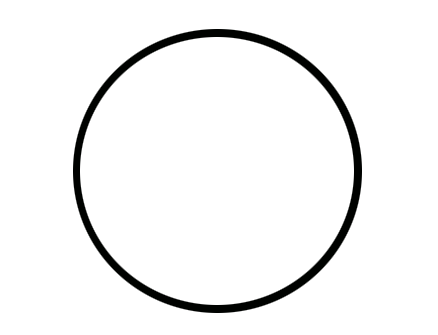
\includegraphics[scale=1.5]{files/premethod/img/dirmap1.png}
	\end{minipage}
	\hspace{0.5cm}
	\begin{minipage}[b]{0.5\linewidth}
		\centering
		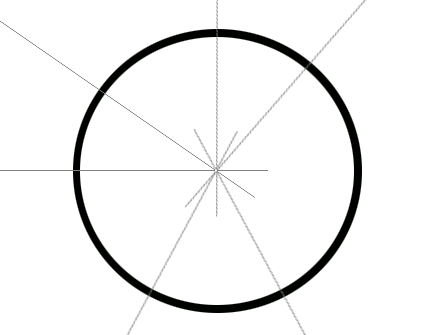
\includegraphics[scale=1.5]{files/premethod/img/dirmap2.png}
	\end{minipage}\\\\
	\begin{minipage}[b]{0.5\linewidth}
		\centering
		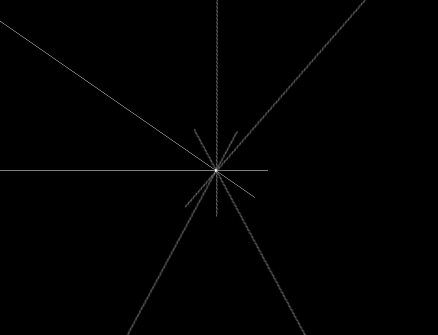
\includegraphics[scale=1.5]{files/premethod/img/dirmap3.png}
	\end{minipage}
	\hspace{0.5cm}
	\begin{minipage}[b]{0.5\linewidth}
		\centering
		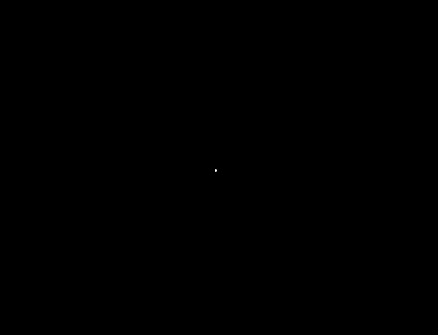
\includegraphics[scale=1.5]{files/premethod/img/dirmap4.png}
	\end{minipage}
	\caption{\textbf{Øverst venstre:} Originale billede. \textbf{Øverst højre:} Cirkel med nogen af linjerne tegnet. \textbf{Nederst venstre:} Det resulterende billede med nogen af linjerne tegner. \textbf{Nedest højre:} Resultat efter tærskelværdi.\label{fig:premethod_houghres}}
\end{figure}

% VORES BILLEDER

\subsubsection{Afledet Gauss-filter}
% fordi?

\subsubsection{Sum of Derived Gaussians}
% Tankegangen med at lave denne

\subsubsection{Foldning med vesikeludsnit}


\subsubsection{Foldning med kantkonkur efter vesikelbillede}
% Ide

\subsubsection{Interverede farver og convolve med billedudsnit} 
% Kant er sort, gøres hvid pga hvid = 255 og nemmere at finde ?

\subsection{Reflektion}
Vi omtalte kort at vesiklerne i figur \ref{fig:premethod_ves1} har forskellige farvet indre. Dette vil vi nu kigge nærmere på. Figur \ref{fig:premethod_vescolors} har indtegnet 3 pile til hver vesikel. Den ene pil peger på vesiklens indre, og de to andre peger på to steder på kanten af vesiklen. 

Tager vi vesiklen til venstre, ses det at der er stor farveforskel på vesiklens indre, og kanten af vesiklen. Det lyseste sted på kanten har stadig en farveværdi på 65 lavere end centrum. En overgang fra kant til centrum er her derfor meget tydelig. Det bemærkes dog også at der er en farveforskel på 33 på det mørkeste og lyseste sted på kanten af vesiklen. 

Tager vi så vesiklen til højre, ser vi at der er en farveforskel på 25 fra det lyseste sted på kanten til det mørkeste. Dette er altså meget det samme som den første vesikel, og farveværdierne ligger da også meget tæt (120 versus 121 for lyseste og 87 versus 96 for det mørkeste). Den store forskel ses når vi tager en pixel fra centrum. Denne har en værdi på 114 (versus 185 i den første) og har altså en farveforskel på kun 7 i forhold til det lyseste sted på kanten.

\begin{figure}[H]
	\centering
	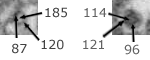
\includegraphics[scale=5]{files/premethod/img/ves_colors.png}
	\caption{Vesikler med 3 farveværdier hver.\label{fig:premethod_vescolors}}
\end{figure}

% hvilket er grunden til at vi ikke kan detektere klare kanter ...

%% Kildeangivelser:
% http://en.wikipedia.org/w/index.php?title=Image_gradient&oldid=421160257
% http://en.wikipedia.org/w/index.php?title=Gaussian_blur&oldid=422700764
% http://en.wikipedia.org/w/index.php?title=Sobel_operator&oldid=422155717